\section{High level design description}
Wir haben den Rechner so entworfen, dass wir die einzelnen Aufgaben möglichst einfach in eigene Module
kapseln können. Dies erleichtert die Implementierung, Wartung und spätere Erweiterung der Module.
Wie diese miteinander kommunizieren wird in folgender Abbildung gezeigt.

\begin{figure}[!ht]
 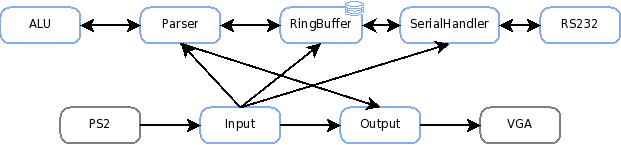
\includegraphics[scale=0.55]{pics/Modules.png}
 % Modules.png: 501x145 pixel, 72dpi, 17.67x5.12 cm, bb=0 0 501 145
 \label{fig:Modules}
\end{figure}

%%%%%%%%TODO Beschreibung der Submodule
\begin{description}
 \item[Input:] Wartet auf Scancodes vom PS2 Modul, bearbeitet diese und schickt, je nach Scancodes, 
ein ASCII Zeichen oder einen Befehle an eine andere Komponente weiter.
 \item[Output:] Bei jedem neuen Zeichen oder nach dem Lösen einer Rechnung muss der Bildschirm aktualisiert werden.
Der Output ist die Schnittstelle zwischen den anzuzeigenden Zeichen und der VGA Komponente, die den Bildschirm 
aktualisiert.
 \item[Parser:] Der Parser wartet auf ein Signal, welches durch das Drücken der Enter Taste ausgelöst wird. Danach holt er sich vom
Ringbuffer Modul die letzte Rechnung, zerlegt diese in seine Grundrechnungen und schickt jede dieser Rechnungen an die ALU.
Nachdem die Berechnung gelöst wurde, wird das Ergebnis an den Ringbuffer und den Output geschickt.
 \item[ALU:] Die ``Arithmetic Logical Unit'' löst die Grundrechnungsarten. Der Parser sendet zwei Operanden und den Operator an die ALU 
und bekommt das Ergebnis zurückgeschickt. 
 \item[Ringbuffer:] Dieses Modul speichert die letzten 50 Rechnungen samt Ergebnissen in einer Ringbuffer Struktur. 
 \item[SerialHandler:] Auf ein Signal vom RS232 oder vom Input Modul holt sich der SerialHandler den gesamten Speicher vom Ringbuffer 
und sendet ihn an die RS232 Komponente.
 \item[RS232:] Dieses Modul hört auf dem RS232 Interface auf den Befehl alle Rechnungen zu schicken und leitet diesen Befehl an den
SerialHandler weiter. Alle Daten die vom SerialHandler kommen werden über das Interface geschickt.
 \end{description}

\subsection{Externe Schnittstellen}
Zwei Schnittstellen bekommen wir fertig compiliert und müssen nicht von uns implementiert werden.
\begin{description}
 \item[PS2:] Das PS2 Modul ist die Schnittstelle zwischen der Tastatur und dem Programm. Jeder Tastendruck sendet 1-3 
Scancodes an unser Input Modul und muss daraus den richtige Befehl interpretieren.
 \item[VGA:] Die VGA Komponente erlaubt einfache Kontrolle über den Bildschirm. Mit mehreren Befehlen kann der Bildschirm
verändert werden.
 \end{description}

\subsection{Reset and Clock}
\begin{description}
\item[Der Reset] wurde low active gewählt.

\item[Der VGA] Controller wird über eine PLL auf 25.175 MHz getaktet. 
Alle weiteren Controller benützen die externe Clockfrequenz
des Developer Boards von 33.33 MHz.
 \end{description}


\subsection{Logical Interfaces}
%Die schon gezeigten Module besitzen folgende I/Os:
%\begin{figure}[!ht]
% 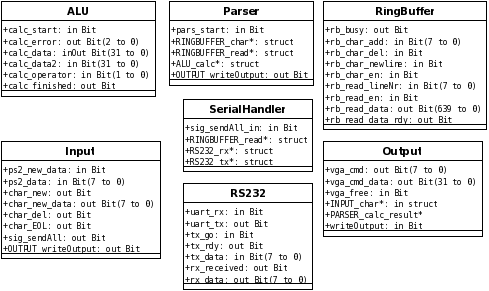
\includegraphics[scale=0.7]{pics/Klassen.png}
 % Modules.png: 501x145 pixel, 72dpi, 17.67x5.12 cm, bb=0 0 501 145
% \label{fig:Klassen}
%\end{figure}

%\subsubsection{Input}

In den folgenden Tabellen 1.1 bis 1.7 stehen zu jeder Komponente die dazu gehörigen
Signale mit Richtung, Bitanzahl und einer kurzen Beschreibung der Signale. 

\begin{table}[h]
 \caption{\textbf{Input Modul}}
 \begin{center}
  \begin{tabular}{|p{4cm}|p{1,6cm}|p{1cm}|p{9cm}|}
   \hline Signal & Richtung & Bits & Beschreibung\\
   \hline
   ps2\_new\_data & in & 1 & Ist High wenn ein neuer Scancode gelesen werden kann.\\
   ps2\_data & in & 8 & Auf diesem Signal liegt der letzte Scancode\\
   inp\_new\_data & out & 1 & Ist High wenn ein neuer gültiger ASCII Code eingegeben wurde.\\
   inp\_data & out & 8 & Der neue gültige ASCII Code.\\
   inp\_del & out & 1 & Beim Drücken der Backspace Taste für einen Zyklus auf High.\\
   inp\_sendRS232 & out & 1 & Wird beim Button auf dem Entwicklerboard ausgelöst.\\
   pars\_start & out & 1 & Beim Drücken der Enter Taste wird der Parser gestartet.\\ 
   \hline
  \end{tabular}
 \end{center}
\end{table}

%\subsubsection{Output}
 
\begin{table}[!h]
 \caption{\textbf{Output Modul}}
 \begin{center}
  \begin{tabular}{|p{4cm}|p{1,6cm}|p{1cm}|p{9cm}|}
   \hline Signal & Richtung & Bits & Beschreibung\\
   \hline
   vga\_command & out & 8 & Befehl an das VGA Modul.\\
   vga\_command\_data & out & 32 & Daten für den Befehl an die VGA.\\
   vga\_free & in & 1 & Signal von der VGA. Erlaubt neue Befehle.\\
   inp\_new\_data & in & 1 & Ist High wenn ein neuer gültiger ASCII Code eingegeben wurde.\\
   inp\_data & in & 8 & Der neue gültige ASCII Code.\\
   inp\_del & in & 1 & Beim Drücken der Backspace Taste für einen Zyklus auf High.\\
   pars\_new\_data & in & 1 & Vom Parser kann ein neuer ASCII Code gelesenw erden.\\
   pars\_data & in & 32 & Der neue ASCII Code.\\
   \hline
  \end{tabular}
 \end{center}
\end{table}

%\subsubsection{Parser}
\begin{table}[!h]
\caption{\textbf{Parser Modul}}
 \begin{center}
  \begin{tabular}{|p{4cm}|p{1,6cm}|p{1cm}|p{9cm}|}
   \hline Signal & Richtung & Bits & Beschreibung\\
   \hline
   ps\_start & in & 1 & Startet Berechnung.\\
   calc\_data & out & 32 & Erster Operand.\\
   calc\_data2 & out & 32 & Zweiter Operand.\\
   calc\_operator & out & 2 & Operator für Berechnung.\\
   calc\_start & out & 1 & Startet Berechnung.\\
   calc\_finished & in & 1 & Berechnung fertig.\\
   calc\_result & in & 32 & Ergebnis.\\
   calc\_status & in & 2 & Status der Berechnung. Bei 0 fehlerfrei, sonst fehlerhaft.\\
   pars\_new\_data & out & 1 & Vom Parser kann ein neuer ASCII Code gelesenw erden.\\
   pars\_data & out & 8 & Der neue ASCII Code.\\
   rb\_busy & in & 1 & Wenn der Buffer beschäftigt ist dürfen keine neuen Eingaben kommen.\\
   rb\_read\_en & out & 1 & Eine neue Zeile wird angefordert.\\
   rb\_read\_lineNr & out & 6 & Die neue Zeile die gelesen werden soll.\\
   rb\_read\_data\_rdy & in & 1 & Die neue Zeile kann gelesen werden.\\
   rb\_read\_data & in & 648 & Die neue Zeile.\\
   \hline
  \end{tabular}
 \end{center}
\end{table}

%\subsubsection{ALU}

\begin{table}[!h]
\caption{\textbf{ALU Modul}}
 \begin{center}
  \begin{tabular}{|p{4cm}|p{1,6cm}|p{1cm}|p{9cm}|}
   \hline Signal & Richtung & Bits & Beschreibung\\
   \hline
   calc\_data & in & 32 & Erster Operand.\\
   calc\_data2 & in & 32 & Zweiter Operand.\\
   calc\_operator & in & 2 & Operator für Berechnung.\\
   calc\_start & in & 1 & Startet Berechnung.\\
   calc\_finished & out & 1 & Berechnung fertig.\\
   calc\_result & out & 32 & Ergebnis.\\
   calc\_status & out & 2 & Status der Berechnung. Bei 0 fehlerfrei, sonst fehlerhaft.\\
   \hline
  \end{tabular}
 \end{center}
\end{table}

%\subsubsection{Ringbuffer}

\begin{table}[!h]
 \caption{\textbf{Ringbuffer Modul}}
 \begin{center}
  \begin{tabular}{|p{4cm}|p{1,6cm}|p{1cm}|p{9cm}|}
   \hline Signal & Richtung & Bits & Beschreibung\\
   \hline
   rb\_busy & out & 1 & Wenn der Buffer beschäftigt ist dürfen keine neuen Eingaben kommen.\\
   pars\_new\_data & in & 1 & Neue Daten von Parser.\\
   pars\_data & in & 8 & Der neue ASCII Code vom Parser.\\
   inp\_new\_data & in & 1 & Neue Daten vom Input\\
   inp\_data & in & 8 & Der neue gültige ASCII Code vom Input.\\
   inp\_del & in & 1 & Ist kurz High wenn ein Zeichen gelöscht werdne soll.\\
   %rb\_char\_add & out & 1 & ??.\\
   %rb\_char\_del & in & 1 & \\
   rb\_char\_newline & in & 1 & Springt in die nächste Zeile.\\
   %rb\_char\_en & in & 1 & \\
   rb\_read\_en & in & 1 & Eine neue Zeile wird angefordert.\\
   rb\_read\_lineNr & in & 6 & Die neue Zeile die gelesen werden soll.\\
   rb\_read\_data\_rdy & out & 1 & Die neue Zeile kann gelesen werden.\\
   rb\_read\_data &out & 648 & Die neue Zeile.\\
   \hline
  \end{tabular}
 \end{center}
\end{table}

%\subsubsection{SerialHandler}

\begin{table}[!h]
\caption{\textbf{SerialHandler Modul}}
 \begin{center}
  \begin{tabular}{|p{4cm}|p{1,6cm}|p{1cm}|p{9cm}|}
   \hline Signal & Richtung & Bits & Beschreibung\\
   \hline
   inp\_sendRS232 & in & 1 & Initialisiert das Senden des gesamten Speichers.\\
   rb\_busy & in & 1 & Wenn der Buffer beschäftigt ist dürfen keine neuen Eingaben kommen.\\
   rb\_read\_en & out & 1 & Eine neue Zeile wird angefordert.\\
   rb\_read\_lineNr & out & 6 & Die neue Zeile die gelesen werden soll.\\
   rb\_read\_data\_rdy & in & 1 & Die neue Zeile kann gelesen werden.\\
   rb\_read\_data & in & 648 & Die neue Zeile.\\
   tx\_rdy & in & 1 & Zum Senden muss rdy low sein.\\
   tx\_go & out & 1 & Startet Sendevorgang.\\
   tx\_data & out & 8 & Das zu sendende Byte.\\
   rx\_recv & in & 1 & Neues Byte wurde empfangen.\\
   rx\_data & in & 8 & Das neue Byte.\\
   \hline
  \end{tabular}
 \end{center} 
\end{table}


%\subsubsection{RS232}

\begin{table}[!h]
 \caption{\textbf{RS232 Modul}}
 \begin{center}
  \begin{tabular}{|p{4cm}|p{1,6cm}|p{1cm}|p{9cm}|}
   \hline Signal & Richtung & Bits & Beschreibung\\
   \hline
   uart\_rx & in & 1 & Die Receive Leitung des UART.\\
   uart\_tx & out & 1 & Die Transmit Leitung des UART.\\
   tx\_rdy & out & 1 & Zum Senden muss rdy low sein.\\
   tx\_go & in & 1 & Startet Sendevorgang.\\
   tx\_data & in & 8 & Das zu sendende Byte.\\
   rx\_recv & out & 1 & Neues Byte wurde empfangen.\\
   rx\_data & out & 8 & Das neue Byte.\\
   \hline
  \end{tabular}
 \end{center}
\end{table}

\subsection{Behavioural Interface}
\subsubsection{Ausgabe am Bildschirm}
Der Bildschirm kann 80 Zeichen in einer Zeile darstellen und unsere Rechnungen können 70 Zeichen lang sein. Mit einem '=' 
Zeichen würden uns 9 Zeichen für das Ergebnis bleiben. Unser Ergebnis ist jedoch 32 Bit lang und liegt zwischen [2147483648,-2147483647].\\
Deswegen und auch wegen der Übersicht schreiben wir das Ergebnis in die nächste Zeile.\\
Der Bildschirmhintergrund ist schwarz mit weißer Schrift. Die Rechnung beginnt in der ersten Zeile. Sollten keine Zeilen mehr 
frei sein rutschen alle Rechnungen um eine Zeile nach oben und die Älteste wird gelöscht.
\subsubsection{Ausgabe über RS232}
Wird der Button am Developer board, oder eine bestimmte Taste am PC, gedrückt, wird der gesamte Verlauf der letzten 50 Rechnungen mit den Ergebnissen an den PC geschickt.
\subsubsection{Umgang mit Overflows}
Overflows werden von unserem ALU Modul abgefangen. Tritt ein Overflow auf wird die Berechnung beendet und eine Fehlernachricht in die History gespeichert.
\subsubsection{Erlaubte Eingabe über Tastatur}
%%%%%%%%%%%%%%%%%%%%%%%%%%%%%%%%%%%%%%%%%%%
%%%Input from detailed design description
%%%%%%%%%%%%%%%%%%%%%%%%%%%%%%%%%%%%%%%%%%%
Das Programm reagiert nur auf gedrückte und nicht auf losgelassene Tasten. Weiters verwenden wir die Scankeys der 
Zahlen und Operatoren vom NumPad und Enter, Leertaste und Backspace von der Haupttastatur.
\begin{center}
\begin{tabular}{|l|l|l|}
\hline ASCII & Scankey (Set2) & ASCII (hex)\\
\hline 0 & 0x70 & 30\\
1 & 0x69 & 31\\
2 & 0x72 & 32\\
3 & 0x7a & 33\\
4 & 0x6b & 34\\
5 & 0x73 & 35\\
6 & 0x74 & 36\\
7 & 0x6c & 37\\
8 & 0x75 & 38\\
9 & 0x7d & 39\\
+ & 0x79 & 2B\\
- & 0x7b & 2D\\
/ & 0xe0 0x4a & 2F\\
$*$ & 0x7c & 2A\\
Backspace & 0x66 & 08\\
Enter & 0x5a & 0A\\
Space & 0x29 & 20\\
\hline

\end{tabular}
\end{center}
\subsubsection{Fehlerhafte Eingaben}
Alle Tasten die nicht spezifiziert sind werden verworfen. Bei fehlerhaften Eingaben wird der Fehler vom Parser und der ALU abgefangen, die Zwischenergebnisse verworfen, die entsprechende Fehlernachricht am Bildschirm ausgegeben und in der History gespeichert.
\subsubsection{Fehlernachrichten}
Wir unterscheiden zwischen drei Fehlernachrichten:
\begin{description}
 \item[Overflow] Wenn bei irgendeiner Berechnung ein Overflow Fehler auftritt. 
 \item[Division durch Null] Sollte bei Irgendeiner Division im Zähler null stehen wird diese Nachricht ausgegeben.
 \item[falscher Syntax]Zu falscher Syntax zählt ein Operand am Ende, zwei Operanden hintereinander oder eine Punktrechnung am Anfang.
\end{description}


\subsection{Physical Interfaces}
Die Physikalischen Interfaces der gesamten angeschlossenen Hardware lässt sich
in nachfolgender Pintabelle ablesen.
\begin{table}[!ht]
 \begin{center}
  \begin{tabular}{|l|l|l|l|}
   \hline Signal & Pin &Direction &Logic Level\\
   \hline
   sys\_clk & N3 & in & LVTTL\\
   sys\_res\_n & AF17 & in & LVTT\\
   btn\_a & A3 & in & LVTTL\\
   uart\_cts & D20 & out & LVTTL\\
   uart\_rts & D21 & in & LVTTL\\
   uart\_txd & D22 & out & LVTTL\\
   uart\_rxd & D23 & in & LVTTL\\
   ps2\_data & E21 & bidirec & LVTTL\\
   ps2\_clk & Y26 & bidirect & LVTTL\\
   vga\_r0 & E22 & out & LVTTL\\
   vga\_r1 & T4 & out & LVTTL\\
   vga\_r2 & T7 & out & LVTTL\\
   vga\_g0 & E23 & out & LVTTL\\
   vga\_g1 & T5 & out & LVTTL\\
   vga\_g2 & T24 & out & LVTTL\\
   vga\_b0 & E24 & out & LVTTL\\
   vga\_b1 & T6 & out & LVTTL\\
   vga\_hsync\_n & F1 & out & LVTTL\\
   vga\_vsync\_n & F2 & out & LVTTL\\
   \hline
  \end{tabular}
 \end{center}
\end{table}

